\chapter{Data Wrangling}
The work discussed in this chapter was done in close collaboration with Dr. Ralf
Seidl, Dr. Francesca Giordano, Daniel Jumper, and Abraham Meles. Eventually the
analysis group merged with another year's analysis group, bringing in Dr. Sanghwa
Park, and Dr. Chong Kim, who have made crucial contributions to this analysis,
and have studied the complimentary 2012 data set, producing their own PhD theses
on this analysis. Dr. Hideyuki Oide has also heavily influenced the techniques
and work-flow of this analysis, pioneering many of the techniques used here (at
PHENIX at least) for his analysis of the 2011 data set.

\label{ch:data_collection}
\section{Overview}
Although we have discussed in detail the theoretical motivations for the W
physics program, as well as the machines producing the necessary collisions and
recording data produced from these collisions, we have not yet addressed the
form of the data set itself, and the substantial engineering it takes to extract
the signal of interest out of that data set.

The relative abundance of the $p + p \rightarrow W^\pm \rightarrow \mu^\pm +
\nu$ signal events is rather low, compared to the other interactions which may
take place when two protons collide. We must allow several hundred million
proton proton collisions to occur, before we have a high probability of
observing just one W-Boson event. 

We discussed in the previous chapter how careful triggering is employed in order
to ensure that any time this event does occur, it is recorded. This does not
guarantee that we \textit{only} record these events. Background events are still
recored much more frequently than signal events, even with the improved
triggering. The number of $W\rightarrow\mu$ events produced over the 2013 data
set number in the hundreds, while the total number of recorded events is
approximately 15 billion.

This leads to the substantial problem of fishing out the appropriate physics
events from the 15 billion event haystack. Why, I hear you ask, don't we just
have a detector which can record only the W-Boson events of interest?

Because, as a multipurpose spectrometer, PHENIX must be ready to take
all kinds of data, and satisfy many experimental requirements, in addition to
fitting a lot of functionality into a relatively tight budget, as is common for
federally funded research. Although this measurement would have been made
much simpler with a forward calorimeter, we can't simply build and install a
calorimeter the moment that an analysis would benefit from its presence.

So, instead, we must rely on our ingenuity and deep understanding of the data
set, to tease out the results we want to measure.

\section{Raw Data to Reconstructed Parameters}

Any time a PHENIX trigger condition is satisfied, all of the information
recorded by the PHENIX spectrometer are read out from temporary on-detector
memory, and fed into a data stream that eventually is archived as a 'PHENIX Raw
Data File Format' or PRDFF. 

PRDFF data is hierarchical, first being organized by event-type, and
then organized by packet-type.  There are many event types - 'DATAEVENTS'
typically carry the information relevant to a physics analysis, whereas other
event-types carry very important QA information for determining the status of
the RHIC apparatus, the beam, polarization, and PHENIX performance.

Every packet has a header, which contains general information such as what the
packet contains, and in what order that packet was received. Every packet
recorded can be associated with a unique event-sequence number, which specifies
roughly the order in which the event owning the packet was received by the DAQ.
Within a given run number, an event-number is guaranteed to be unique. The
complexity of the packet is limited by the bandwidth available to move data off
PHENIX onto other storage, and the buffers/reconstruction ability of the front
end electronics modules built onto PHENIX subsystems. PHENIX archives data from
the DAQ at a rate of approximately 700 Megabytes per second - or one compact
disk.

Generally, raw PHENIX data is too complex to use straight-away, because minimal
to no reconstruction of physical properties for a certain event is done, due to
hardware limitations and time limitations - some of this raw data is often
directly used in triggering decisions, which must be made once every 106
nanoseconds or faster (the bunch crossing frequency).

The raw data collected from PHENIX undergoes a process called "Data Production",
where physical parameters are reconstructed from the simpler raw data. Raw data
could take any form - for example - which cathode strips were activated in an
event in the muon tracker, or, the number of photons counted in a
photomultiplier tube. This information is often combined with extensive survey
information about the geometry of a given detector, the known magnetic field in
a detector, to reconstruct quantities such as momentum, or deposited energy.

Once reconstruction has finished in a Data Production, the data are then
repackaged into ROOT files, often times internally structured into custom output
objects which are associated with a various detector. These output objects are
simply custom written C++ classes which have a serialization scheme, which have
libraries and dictionaries compiled that allow for them to be serialized into
ROOT's file format.

For the purposes of this analysis, all data has been reconstructed and
serialized into a specific type of output object called a 'picoDST' or even more
concisely, 'pDST'. This name, like many others in PHENIX has historical context:
DST stands for 'Data Summary Tape' hearkening back to the days when data was
stored primarily on magnetic tape (it is still archived on magnetic tape!), and
'pico' because of its relatively small disk-space requirement, compared to
'nanoDST' files or simply 'DST' files. I'm not making this up, I swear!

\section{Choosing Analysis Variables}

Even data reduced to the point of a pDST still is much more complicated and
comprehensive than what is needed for this analysis - there are thousands of
variables relating to reconstruction parameters. We only need a handful of
variables for this analysis, summarized on Tables
\ref{tab:evt_variables},\ref{tab:mutr_variables}, \ref{tab:fvtx_variables} and
\ref{tab:rpc_variables}. When Cartesian coordinates are referenced, implicitly,
the reference frame is the PHENIX Coordinate system
(Figure~\ref{fig:phenix_coordinate_system}).

As you can probably guess, the only variables which are truly relevant to this
analysis need to be relevant to understanding two questions:

\begin{enumerate}
  \item \textit{Is this reconstructed muon track the result of a real W-Boson Decay?}
  \item \textit{What is the polarization of the two colliding protons for every recorded collision?}
\end{enumerate}

To properly answer these questions, we need to comprehensively understand what
processes are capable of producing muons, as well as whether or not our detector
can be 'tricked' by signals which look like muons, but really aren't. Secondly,
we need a means of recovering the proton spin polarization for each colliding
bunch-pair.

Polarization recovery is straight-forward - we already have mechanisms in the
data stream which number and track the colliding bunch pairs. We additionally
have well defined spin patterns which are applied to the 120 bunches, the same
way every time this pattern is applied to the fill. As discussed previously, we
have good QA apparatuses in place to ensure the advertised spin pattern is the
same as the delivered spin pattern. Since polarization patterns do not typically
change in a standard physics beam fill (if they do, alarms are raised and the
data is typically discarded), all that is needed is to associate a PHENIX run
number, with a RHIC fill number, and then look up the spin pattern, which in
effect, is a database-call. Of course, the overall beam polarization percentage
is an important factor, which dilutes any spin asymmetry, but this is taken into
account in the final spin database QA analysis~\cite{Kim2014}.

So, effectively we really only need to answer the first question for this
analysis. And the difficulty in answering this question is essentially that it
is very difficult to differentiate signal $W\rightarrow\mu$ events from other
$X\rightarrow\mu$ events, or even events which look like muons, but are really
due to incorrect track reconstruction.

So, the thrust of the Data Analysis portion of this work is really just to tease
apart the real W-genic muons, from all other muon candidates. To this requires
some substantial feature engineering, and creating some statistical models, as
well as a means of evaluating the performance of these statistical models -
which is difficult because validating any statistical differentiation technique
(aka machine learning technique) requires a labeled data set, and we
intrinsically do not possess this, since otherwise, this analysis would not need
to be done.

\begin{table}
  \centering
  \begin{tabular}{l p{0.7\linewidth}}
    \toprule
      \textbf{Name} & \textbf{Description} \\
    \midrule
      Run\_Number & A unique number identifying a run in a RHIC fill for PHENIX \\
      Evt\_Number & A unique number within a single run identifying the approximate order an event was taken. \\
      Evt\_bbcZ & The event z-vertex calculated by the BBC \\
      triggerbit & The result of a bit-wise 'OR' applied to all 32-bit trigger bits which fired \\
    clockcross & The bunch number of the two colliding bunches $[0-119]$. Required to look up the spin polarization, along with Run\_Number \\
    \bottomrule
  \end{tabular}
  \caption{Variables characterizing events overall}
  \label{tab:evt_variables}
\end{table}

\begin{table}
  \centering
  \begin{tabular}{l p{0.7\linewidth}}
    \toprule
    \textbf{Name} & \textbf{(Unit) Description} \\
    \midrule
    Evt\_Nmu & The number of muon tracks reconstructed for a given event \\
    charge & ($\pm e$) The charge associated with a reconstructed muon track \\ 
    $p_z$ & (GeV) The z-momentum associated with the muon track \\
    $p$ & (GeV) The total momentum of a charged track \\
    $\chi^2$ & The result of the Kalman fitter reconstructing the track \\
    lastGap & The last gap in the Muon Tracker which was activated (there are 4) \\
    $\eta$ & The rapidity of the track \\
    $\phi$ & (rad) The azimuthal position angle the track makes relative to the x-axis \\
    DG0 & (cm) A Track matching variable (matching between MuID and MuTR) associated with the MuID road, at MuID station 3. \\
    DDG0 & (degree)  The opening angle between the MuID track road, and the MuTr projection onto the MuID \\
    xSta${}_i$ & (cm) The x-coordinate of the track at Station i,  $i\in{1,2,3}$ of the MuTr \\
    ySta${}_i$ & (cm) The y-coordinate of the track at Station i, $i\in{1,2,3}$ of the MuTr \\

    $\phi_i$ & (rad) The angle the track makes with Station i, $i\in{1,2,3}$, i.e.: $\phi_i = tan^{-1}\left({{x_1}\over{y_i}}\right)$ \\
    $\theta$ & (rad) Azimuthal angle of track, $tan^{-1}\left({p_T \over p_z}\right)$ \\
    DCA${}_z$ & (cm) Distance of closest approach between the z-vertex positions extracted by projecting the MuTR track z-vertex back to the BBC z-vertex \\
    DCA${}_r$ & (cm) Distance of closest approach between the track and beam axis \\ 
    \bottomrule
  \end{tabular}
  \caption{
    Muon tracker variables. Generally, this data set is indexed on a subevent 
    level, where one event will contain all reconstructed muon tracks seen for 
    that event.
  }
  \label{tab:mutr_variables}
\end{table}

\begin{figure}
  \centering
  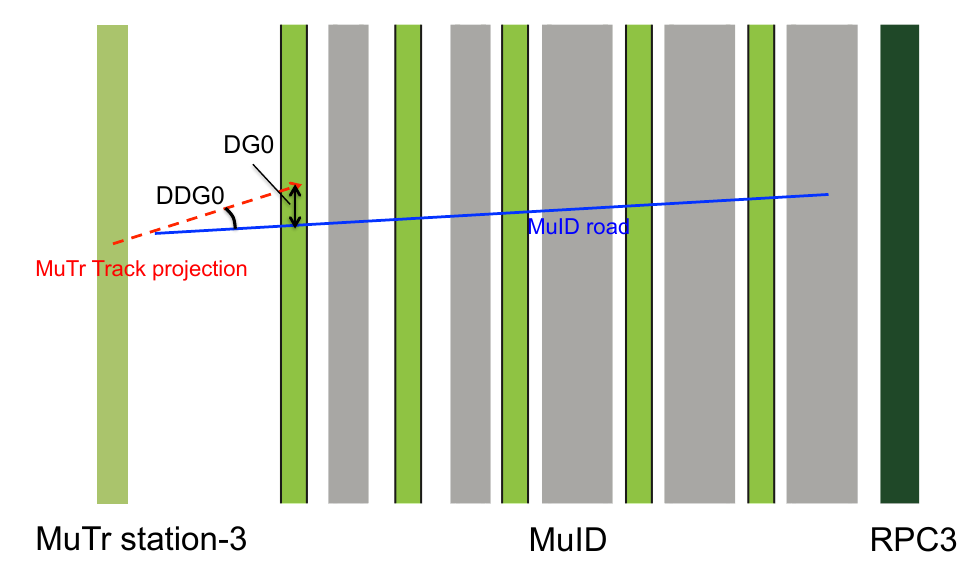
\includegraphics[width=0.7\linewidth]{./figures/dg0_ddg0.png}
  \caption{
    A schematic representation of the matching variables, DG0 and DDG0 at
    the intersection between the Muon Tracker and Muon 
    Identifier~\cite{Oide2012}
  }
  \label{fig:dg0_ddg0}
\end{figure}

\begin{table}
  \centering
  \begin{tabular}{l p{0.7\linewidth}}
    \toprule
    \textbf{Name} & \textbf{Description} \\
    \midrule
    $fvtx_{d\phi}$ & The $\phi$ residual between MuTR track and FVTX track \\
    $fvtx_{d\theta}$ & The $\theta$ residual between the MuTR track and FVTX track \\
    $fvtx_{dr}$ & The radial residual between the MuTR track and the FVTX track \\
    $fvtx_{conebits}$ & The number of FVTX clusters inside a cone around the track defined by: $0.04 rad < dR < 0.52 rad$ where $dR = \sqrt{{d\eta}^2+{d\phi}^2}$\\
    \bottomrule
  \end{tabular}
  \caption{A summary of the variables reconstructed from FVTX raw data~\cite{Meles2015}.}
  \label{tab:fvtx_variables}
\end{table}

\begin{table}
  \centering
  \begin{tabular}{l p{0.7\linewidth}}
    \toprule
    \textbf{Name} & \textbf{Description} \\
    \midrule
    RpcMatchSt1 & Distance of closest approach between projected MuTR track onto the RPC 1 and the closest hit cluster on RPC 1\\
    RpcMatchSt3 & Distance of closest approach between projected MuTR track onto the RPC 3 and the closest hit cluster on RPC 3\\
    \bottomrule
  \end{tabular}
  \caption{RPC Track matching variables}
  \label{tab:rpc_variables}
\end{table}

\begin{figure}
  \centering
  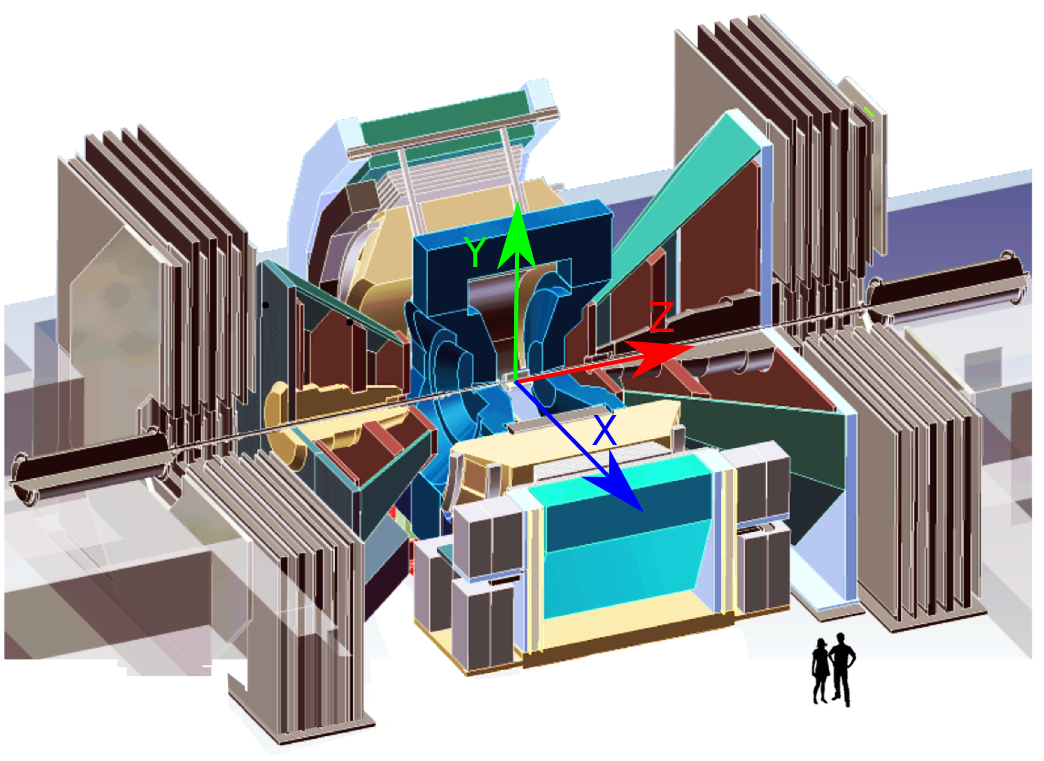
\includegraphics[width=\linewidth]{./figures/phenix_coordinate_system.png}
  \caption{
    The PHENIX coordinate system is shown (RGB arrows) at the center of the
    nominal interaction point within PHENIX, the origin, in this quarter-cutaway
    drawing. The small black figures are actually miniaturized human beings, the
    PHENIX detector is very small - this is a full scale drawing of PHENIX.
    Shown: the x, y, and z coordinates, as well as the azimuthal coordinate,
    $\theta$ and polar coordinate $\phi$ ~\cite{WebPHENIXDrawings}
  }
  \label{fig:phenix_coordinate_system}

\end{figure}


\begin{figure}
  \centering
  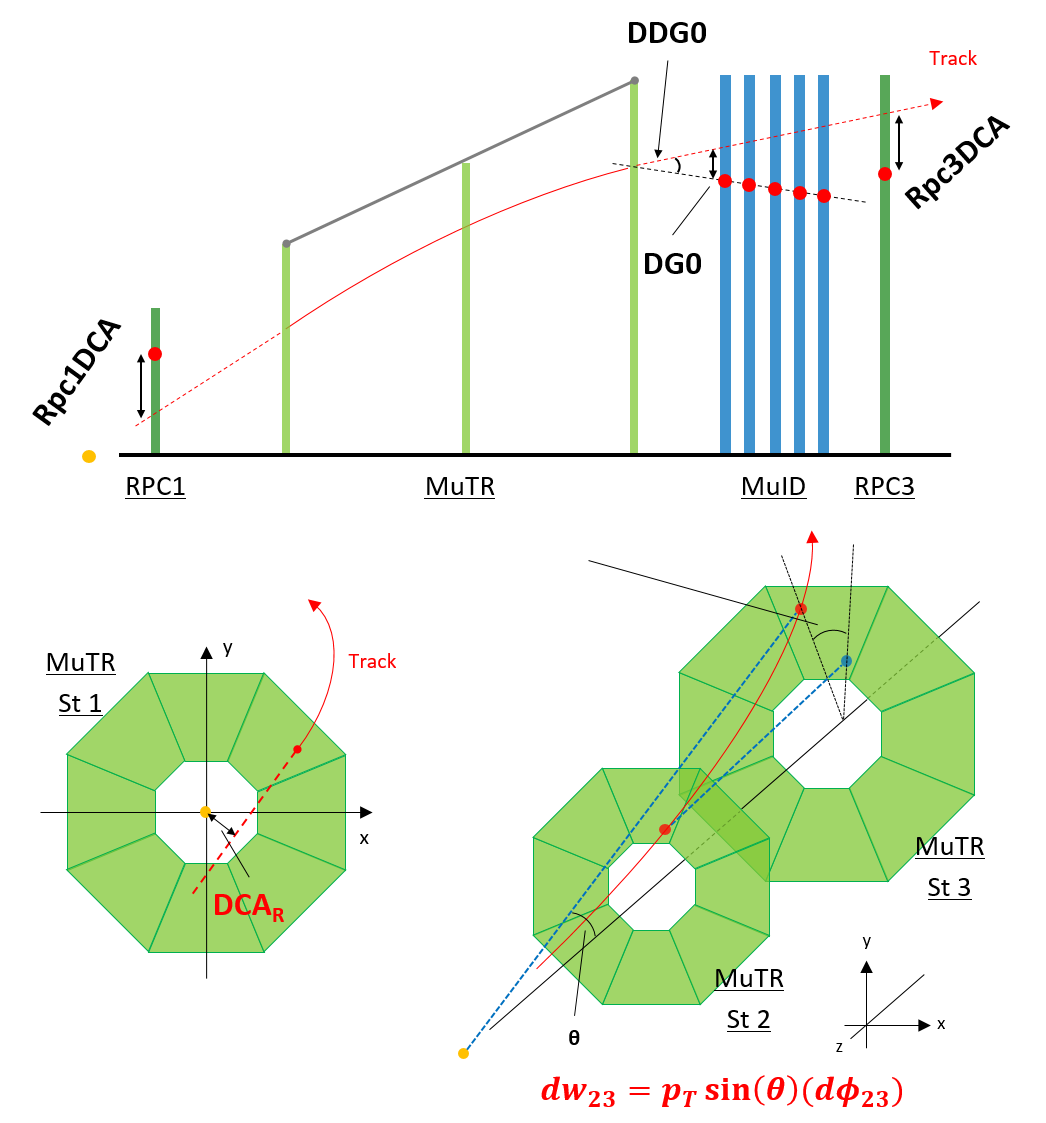
\includegraphics[width=0.8\linewidth]{./figures/kinematic_variables_schematic.png}
  \caption{
    A nice summary of discriminating kinematic variables reproduced with
    permission from Dr. Chong Kim. We see tracking planes in green, and a muon
    track penetrating the planes in red, and reference coordinates in the lower
    right-hand corner.
  }

\end{figure}

We engineer some variables as well, in addition to those that we have explicitly
extracted from the reconstructed physics data. These variables play an important
role in our extraction of the signal to background ratio. They are: $dw_{13}$,
$dw_{23}$, d$\phi_{13}$, d$\phi{23}$. The $d\phi_{ij}$ variables represent the
difference in azimuthal angle observed at the MuTR station i and j respectively.
$dw_{ij}$ is constructed from $d\phi_{ij}$ as follows:
\begin{equation}
  dw_{ij} = p_T \times sin(\theta) \times d\phi_{ij}
  \label{eq:dw23_definition}
\end{equation}

While $\phi_{i}$ is calculated from the x and y coordinates at Station i:

\begin{equation}
  \phi_i = tan^{-1}\left({ySta_i \over xSta_i}\right)
  \label{eq:phi_definition}
\end{equation}

A common theme amongst these variables is that they should help us distinguish
between high momentum muon tracks from W-Bosons, and other muon tracks. The hope
is that the muon tracks from W-Bosons are kinematically restricted to have a
relatively narrow momentum distribution in the forward kinematic regime, and so
therefore, tracking variables can be used to partially differentiate between
signal and background events.

In general, W-genic events will be mostly straight, geometrically, and so this
constrains the values of variables such as DCA${}_r$ substantially, and other
variables less so.

Our secondary requirement of our variables is that they are relatively
uncorrelated with each-other, to leave plenty of room for statistical modeling.
Ultimately, we chose a subset of the available tracking variables to carry out
the analysis, in two stages.

In the first stage of the analysis, we use: DG0, DDG0, DCA${}_r$, $chi^2$,
Rpc1DCA, Rpc3DCA, $fvtx_{dr \times d\theta}$, $fvtx_{d\phi}$, and $fvtx_{cone}$.
Of these variables, some were grouped to account for correlations: DG0 and DDG0,
$\chi^2$ and DCA${}_r$. These variables are all related to track reconstruction.
The Muon Tracker reconstructs tracks by essentially connecting the dots between
x and y coordinate 'hits' that it records at each station. The lines connecting
these hits are called 'roads'. Following this, the roads and hits are used to
generate a curve fit to the data, given knowledge of the muon tracker's radial
magnetic field. From this curve, we extrapolate the charge and momentum, and we
construct variables which codify the difference between the reconstructed curve,
and the 'connect the dots' roads. The smaller these differences are, the more
straight the track is, and as discussed, straightness points to higher momentum,
which ultimately leads to labeling as a W-genic particle, if the momentum is in
the correct range.

In the second phase of the analysis, we use $dw_{23}$ and $\eta$ primarily. Both
stages of the analysis are discussed in the following sections. $dw_{23}$ is
related to track straightness as well, and is referred to as "reduced azimuthal
bending". Since we're interested in forward muons, $\eta$ is used as our second
variable.

Generally, we are interested in recovering forward $\mu+$, forward $\mu-$,
backward $\mu+$ and backward $\mu-$. As the muon arms do not have the same
rapidity coverage, we separate the data into these four categories - forward
positive charged tracks, forward negatively charged tracks, backwards positively
charged tracks and backward negatively charged tracks. Due to the geometry of
the muon arms, the North Arm will always correspond with forward positive
rapdity, whereas the South Arm will always correspond with backward, negative
rapidity. I will use 'forward and backward' interchangably with 'North and
Sout'. We perform all calculations with our data set in parallel between these
four conditions.

The data is further subdivided based on the available track matching variables
for a given event, but these subdivisions are not kept separate from the
overall arm-charge separation. Some variables, such as the RPC track matching
variables and the FVTX track matching variables exist for some events, but not
others. We will discuss how this is managed in later sections, but this data is
not generally partitioned in this way.

\clearpage
\section{Feature Engineering}
The ultimate goal of Feature Engineering is to clean the data and transform the
data with heuristic strategies that tag events coming from signal sources, as
separate from events which come from our background, so that we can proceed with
the calculation of the physics asymmetry.

Even with the Forward Upgrade (Section~\ref{sec:foward_upgrade}), our data set
is still composed mostly of background events
(Figure~\ref{fig:data_composition}). The primary constituents of the data set
are muons from the following sources:

\begin{itemize}
  \item \textbf{Hadronic Background}
    \begin{itemize}
      \item The hadronic background is composed of hadrons which are produced
        from the primary event vertex, and then travel into the muon arms. The
        hadrons then decay in the muon arms, and create hits at each station,
        which are mis-reconstructed as high-$p_T$ muons.
    \end{itemize}
  \item \textbf{Muon Background}
    \begin{itemize}
        \item The muon background is composed of processes which produce real
          muons which fall into a similar kinematic regime of the W-genic muons
    \end{itemize}
  \item \textbf{W Signal}
    \begin{itemize}
        \item These are muons we are looking for. They come from the W boson
          decay, and carry information about the proton spin.
    \end{itemize}
\end{itemize}

We will differentiate these types of data in two different step. In the first
step, we will use likelihood event selection, where we lump hadronic background
and muon background together, and merely distinguish it from W-genic events. In
the second stage, we will further differentiate our model for the background,
drawing heavily on the data to understand the hadronic background, and providing
simulations of the W-genic events as well as simulation cocktail for other muon
background events. Before we discuss this differentiation, it is important to
discuss the simulations, as the rest of the analysis hinges on the simulation of
both the W-genic events and the Muon Background events.

\begin{figure}[ht]
  \centering
  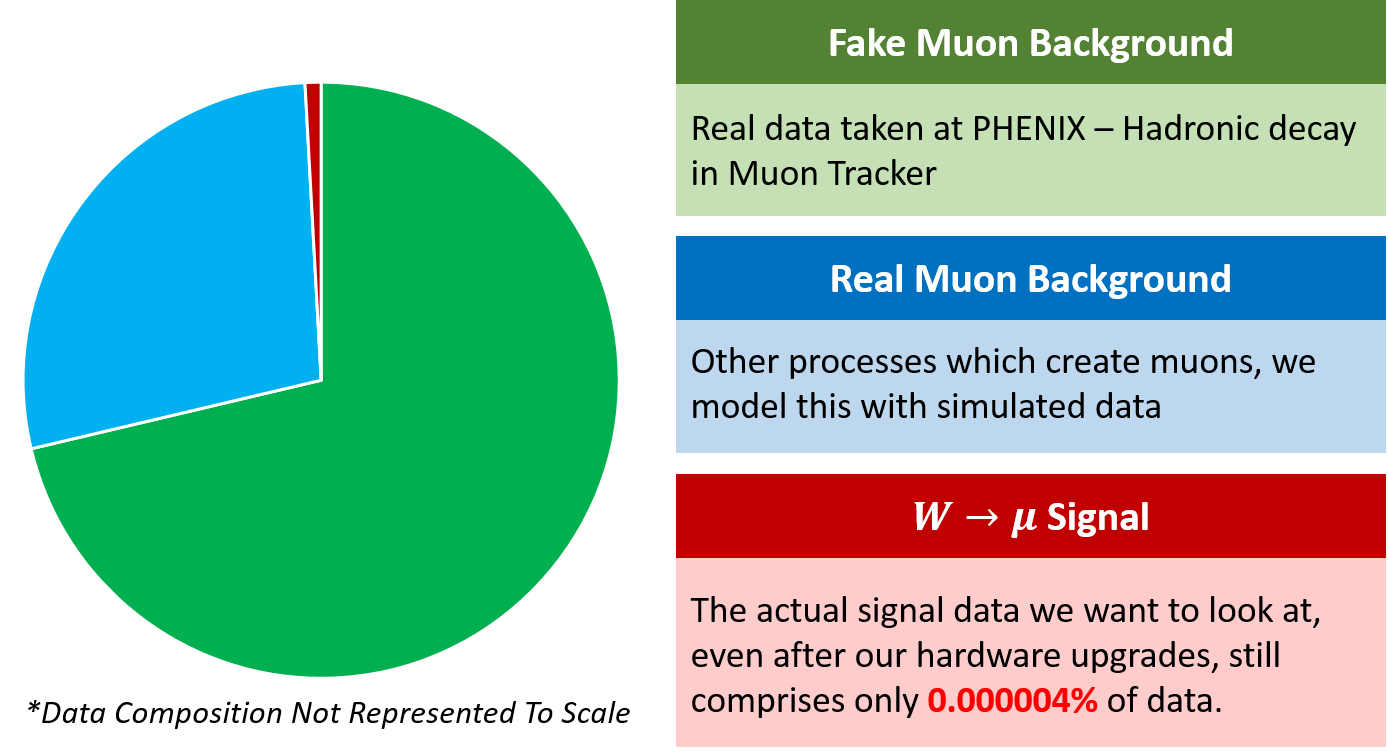
\includegraphics[width=0.8\linewidth]{./figures/data_composition.png}
  \caption{
    A cartoon of the dataset composition. The data, even after the Forward
    Upgrade, is mostly composed of hadronic background, which has tricked our
    Muon Tracker.
  }
  \label{fig:data_composition}
\end{figure}

In subsequent sections, I will discuss what we do with the variables which we
have chosen to use to identify W-genic events. Because our data set is so
dominated by background sources, we must rely heavily on simulations to estimate
what our signal events might look like. As of the time of this writing, the
analysis has not yet incorporated the simulation of hadronic background, which
is quite difficult, as there are a lot of effects at play - particles which
interact with the material of PHENIX itself to produce secondary and tertiary
vertices, for example. However, if we can simulate accurately the signal process
(the W-Boson cross section and its scaling with energy is known to excruciating
precision), and the muon background processes (known to similarly high
precision), we can approach the problem from a standpoint of using our data set
as a relatively good model for what 'hadronic background' looks like, and use
simulations to fit the portions of the data which cannot come from this hadronic
background. 

\clearpage
\subsection{The Basic Cut}

The basic cut aims to remove all obviously bad events from our event mix. The
cut approaches this from two premises. The first, is that if track
reconstruction variables simply cannot have resulted from a W-genic event, then
we remove the track. Secondly, if the track corresponds to a reconstructed
energy which is larger than what is physically allowable for a W-genic track, we
remove it.

The "Basic Cut" is defined:
\begin{table}[ht]
  \centering
  \begin{tabular}{l c c}
    \toprule
    \textbf{Variable} & \textbf{Lower Bound} & \textbf{Upper Bound} \\
    \midrule
    MuID lastGap & * & Gap 4 \\ 
    $\chi^2$ & 0 & 20 \\
    $DG0$ & 0 & 20 \\
    $DDG0$ & 0 & 9 \\
    $\mu$ candidate & * & 1 \\
    \bottomrule
  \end{tabular}
  \caption{ The Basic Cuts used in the Run 13 analysis. lastGap refers to the
    last gap in the MUID which saw a $\mu$ candidate event. The fourth gap is
    the furthest penetration possible, therefore suggesting a high energy muon.
    Other parameters are described in Tables \ref{tab:evt_variables}, 
    \ref{tab:mutr_variables}, \ref{tab:fvtx_variables}, and
    \ref{tab:rpc_variables}
  }
  \label{tab:basic_cut}
\end{table}

With this cut, we have removed quite a large fraction of the data, without worry
of removing signal events.

\clearpage
\subsection{Simulations}

I did not do any work to produce the simulations used in this analysis, all of
that credit goes to Dr. Ralf Seidl. I will generally describe how the
simulations were produced, and paraphrase from the analysis note which we
co-wrote with contributions also from Dr. Giordano, Abraham Meles and Daniel
Jumper:~\cite{Seidl2014}.

PHENIX has a rather well developed simulation framework, which uses the in-house
built "PHENIX Integrated Simulation Application" (PISA)~\cite{Macguire1997}
custom simulation framework. The simulation framework models in great detail the
entire 12mx18mx18m volume of the PHENIX apparatus, as well as all the various
material properties of the apparatus. The software package originated from the
GEANT geometry and tracking packages. PISA encompasses more than this, though,
it additionally encapsulates event-generators, a standalone geometry
verification package, and the PHENIX offline analysis shell, to generate data
that is completely compatible with PHENIX's data packaging framework. PISA has
since been integrated into a simulation work-flow with the popular PYTHIA event
generation system.

The simulations were created by selecting the biggest sources of muon
background known to be produced at PHENIX as well as the W-Boson event and
producing many events to generate good statistics. The primary purpose of
simulating the muon background and W-Signal is to ultimately generate
probability distribution functions for the variables which have the largest
analyzing power - i.e. ability to differentiate between signal and background.
The simulation and data both are ultimately described by the same variables.

The data are added together, when combined to generate a 'muon background pdf'
or 'W-Signal pdf' according to the cross-section of the process and the number
of generated events, so as to not add these ingredients into the cocktail in the
wrong amounts. This process is described in the next section, but the
simulations used in this analysis are summarized here, in
Table~\ref{tab:simulation_cross_sections}. When adding the simulations together,
one must be careful to scale the final-yields by a correction factor (called
k-factor) such that events which produce boosted dimuons are properly accounted
for.

PHENIX uses some somewhat exclusive jargon when describing the various quark
bound states which contribute to the muon background, and signal events.  Open
charm or charmonium refer to the bound state of the $c\bar{c}$ quarks.  Onium
generally refers to any process where a particle is in a bound-state with its
own antiparticle (without of course double-counting open charm/charmonoim).
Direct photon, or alternatively $d\gamma$ (sometimes also written as DY) refers
to photons that are produced as an immediate result of a inelastic scattering
process, not from secondary decays. Open bottom refers to the bound state of
$b\bar{b}$ quarks. Z/$d\gamma$ refers to the production and decay of the mixing
between the Z-boson and virtual photons. ONLY Z refers to Z production and
decay.  W is naturally the signal event. W tau refers to the production of tau
leptons, which can decay weakly, producing electrons or muons. W had refers to
the production of W bosons from hadronic processes, rather than as the primary
event vertex.  All of these processes are summarized in
Table~\ref{tab:simulation_cross_sections}.  
\begin{table}[ht]
  \centering
  \begin{tabular}{ccccc}
    \toprule
    \multicolumn{5}{c}{\textbf{Reference Run 393888}}\\ 
     & & & & \\
    \textbf{Process} & 
    \textbf{k factor} & 
    \textbf{$\sigma$ } & 
    \textbf{\# Events} & 
    \textbf{ $\mathcal{L}$ } \\
    & & (\textit{mb}) &  & ($fb^{-1}$) \\
    \midrule
    $c\bar{c}$ & 1.5 & 5.71e-01 & 5.85e+11 & 1.02\\
    onium      & 1.5 & 1.35e-01 &  1.5e+11 & 1.11\\
    $d\gamma$  & 1.5 & 5.32e-02 & 5.84e+10 & 1.10\\
    $b\bar{b}$ & 1.5 & 7.30e-03 & 7.36e+09 & 1.01\\
    ONLY Z     & 1.5 & 3.37e-07 & 1.73e+08 & 577.0\\
    W          & 1.5 & 1.66e-06 & 3.38e+08 & 198.9\\
    W tau      & 1.5 & 1.66e-06 & 3.43e+08 & 201.8\\
    W had      & 1.5 & 1.66e-06 & 3.42e+08 & 201.2\\
    Z          & 1.5 & 1.02e-06 & 2.93e+08 & 61.2\\
    \bottomrule
  \end{tabular}
  \caption{
    Simulated sub processes in Run 13 including their generated event numbers
    as well as the corresponding luminosity and cross sections.
  }
  \label{tab:simulation_cross_sections}
\end{table}                  

We can visualize the composition of the simulated data set by stacking the
relative distributions of these variables. By looking the cross-sections of
these variables as a function of $p_T$, for each arm and charge combination, we
can get a feeling for how the data set composition varies with $p_T$
(Figure~\ref{fig:stacked_xsec_sim}).

\begin{figure}[ht]

  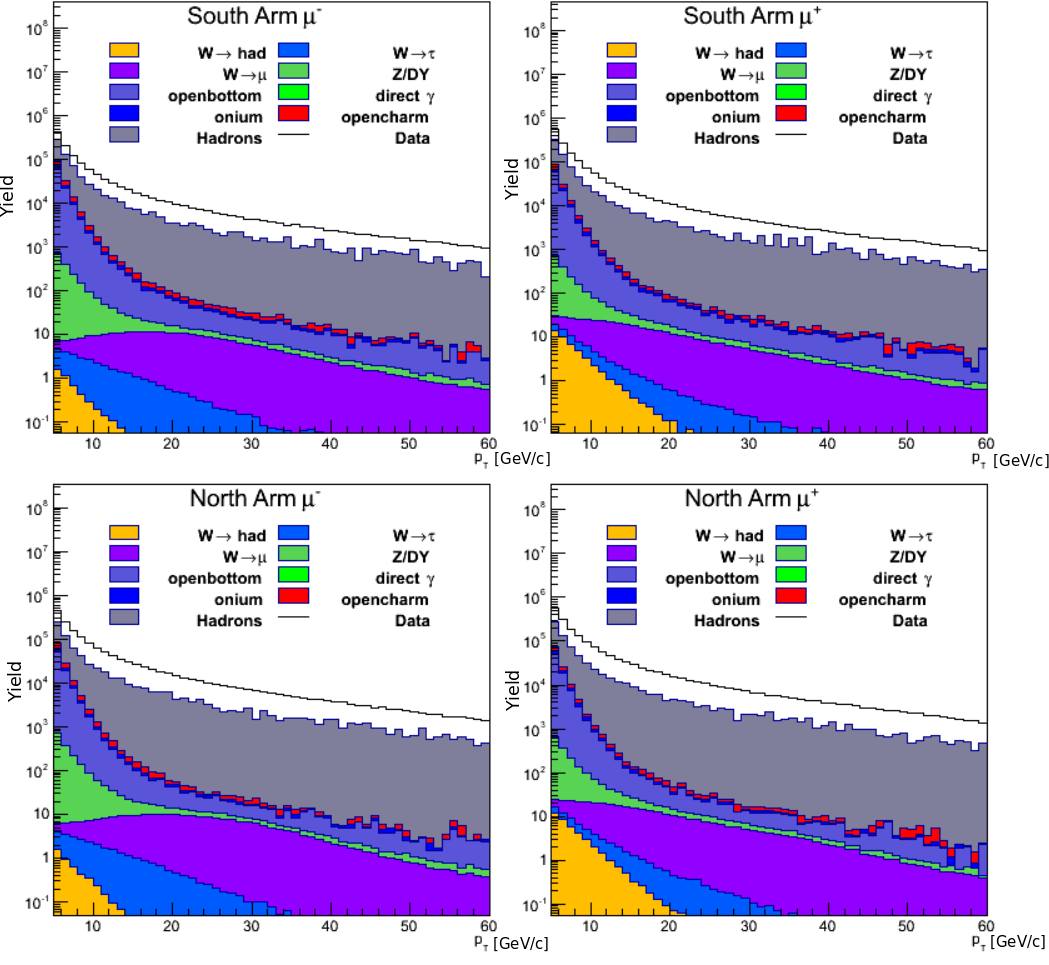
\includegraphics[width=\linewidth]{./figures/stacked_xsec.png}
  \caption{
    Here, we see the stacked cross-sections of all simulated processes as a
    function of $p_T$. All data shown has been created from the PISA+PYTHIA
    framework. Top Left: South $\mu-$, Top Right: South $\mu+$, Bottom Left:
    North $\mu+$, Bottom Right: North $\mu-$  ~\cite{Seidl2014}
  }
  \label{fig:stacked_xsec_sim}
\end{figure}

\clearpage


\subsection{$W_{ness}$: Likelihood Event Tagging}
\label{sec:likelihood}

Recalling that we have already split the dataset into three main contributions:
hadronic background, real muon background, and W-Signal, we are now tasked with
formulating a means to separate signal from background, using the variables
which can indicate the straight-ness of a muon track.

Previous analyses have attempted to separate the muon spectrum into $p_T$ bins,
to estimate the composition, however, because the $W\rightarrow\mu$ signal is so
small in the forward kinematic regime, these methods are not sufficient, as
there is no 'visible' cutoff in the spectrum.

However, we may use other methods to split up our spectrum, with the ultimate
goal of calculating $A_L$, and correcting for background dilution using the
signal to background ratio. We must use another method to effectively describe
the difference between an event which comes from a signal, vs background event.

We expect that tracks which are straight are more likely to come from a W-Boson
decay, because this indicates high momentum. One way of thinking of our data set
can in terms of a classification problem. In a classification problem, one can
use Bayes Theorem when one has a labeled testing data set to build predictive
models which can classify data into two or more classes, provided that care is
taken to not over-train the classifier, or attempt to classify data which has
been used in the subset of data to train the classifier.

In our case, we have simulations which serve as the training data, guaranteeing
that there will be no overlap between the physical data produced, and the data
used to train the classifier. Thus, we implement a Naive Bayes Classifier (also
known as Likelihood Selection) to label our data with two classes. Rather than
labeling data with a binary classification, however, we opt to label the data
with its likelihood, a posterior probability which tells us if a value is more
or less likely to come from a W-Boson.

\subsubsection{Naive Bayes Classification}
There are many techniques available for classifying a collection of variables
(a feature set) into categories. Naive Bayes classification is an excellent
candidate for classification, in cases where we have two classifications with
distributions of feature sets which are uncorrelated. Naive Bayes even works when
feature sets are slightly correlated. It is a robust, fast, scalable machine
learning technique. Traditionally used for classification of text documents,
Naive Bayes is also able to handle numeric features whose distributions are
known \cite{Collins2013}.

In our analysis, we begin with a Naive Bayes classifier which is trained to
classify signal muons or background muons. We combine both Real Muon
Background muons and Fake Muons (Hadronic Background Muons) in the label of
"Background Muons" at this stage, though, later, we will separate out the muons
further.

In order to obtain the best performance from our classifier, without
over-training, we need to ensure that the variables (or feature set) used to
determine a class are maximally uncorrelated. The variables which match this
criteria are: DG0, DDG0, $\chi^2$, $fvtx$ variables, Rpc1DCA, Rpc3DCA, DCA$_r$,
and DCA$_z$. The Linear Correlations between these variables are shown for both
the data, and the simulated W-Signal in
Figure~\ref{fig:kinematic_var_correlations}.

\begin{figure}[H]
	\centering
	\begin{subfigure}[t]{0.5\textwidth}
		\centering
		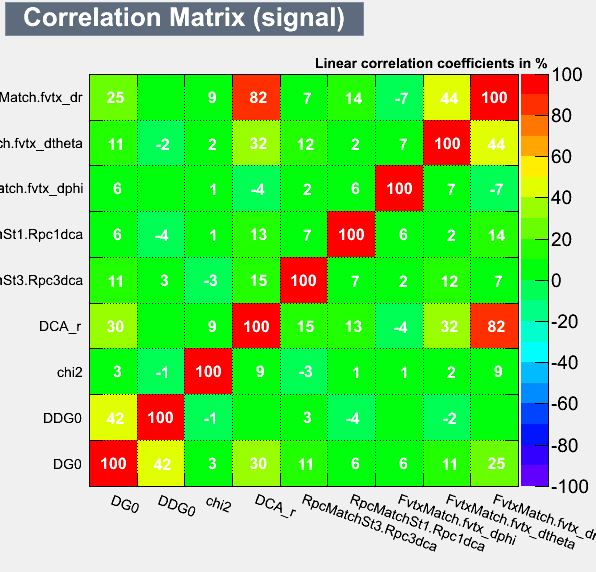
\includegraphics[width=0.95\linewidth]{./figures/CorrelationMatrix_Signal.png}
		\caption{Correlations between kinematic variables, produced from simulated
			data.}
		\label{fig:corr_mat_sig}
	\end{subfigure}%
  \begin{subfigure}[t]{0.5\textwidth}
		\centering
		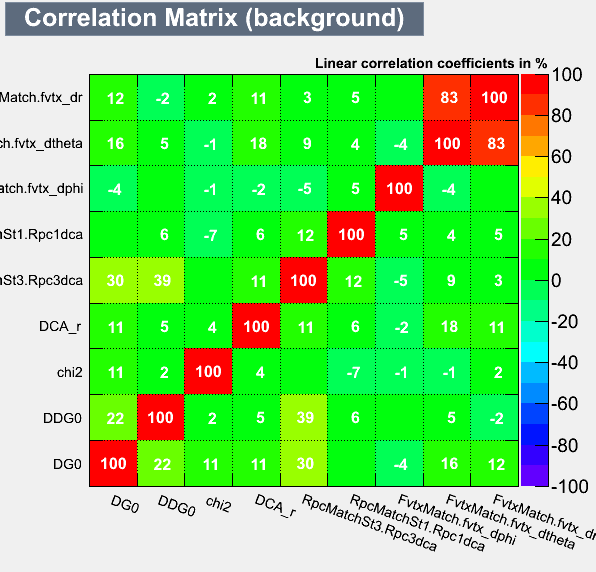
\includegraphics[width=0.95\linewidth]{./figures/CorrelationMatrix_Background.png}
		\caption{Correlations betwen kinematic variables, produced from the data,
			which is composed mostly of hadronic background}
		\label{fig:corr_mat_bkg}
	\end{subfigure}
	\caption{ Low correlations between the signal variable distributions (from
		simulation), and the background variable distributions make this data set a
		good candidate for classfication using Naive Bayes}
	\label{fig:kinematic_var_correlations}
\end{figure}

As one can see from Figure~\ref{fig:kinematic_var_correlations}, DG0 and DDG0
are slightly correlated, as are $chi^2$ and DCA$_r$. A Naive Bayes classifier
may be constructed from the core of the familiar Bayes Theorem from probability
and statistics. In our case, we understand Naive Bayes as a conditional
probability. Concretely, we consider a vector of features (i.e.  our
discriminating kinematic variables):

\begin{equation}
	\label{eq:feature_vector}
\mathbf{x} = (x_1, \dots, x_n)
\end{equation}

and assume independence between each feature $x_n$. We then define the
probability of a given classification, $C_k$ given a set of features $x_n$:

\begin{equation}
	\label{eq:cond_probabilty}
  \mathcal{P}(C_k \vert x_1, \dots, x_n)
\end{equation}

This conditional probability is defined in terms of Bayes Theorem:

\begin{equation}
	\label{eq:bayes_theorm}
  \mathcal{P}(C_k \vert \mathbf{x}) = \frac{\mathcal{P}(C_k) \
  \mathcal{P}(\mathbf{x} \vert C_k)}{\mathcal{P}(\mathbf{x})}
\end{equation}

The terms here are defined as:
\begin{itemize}
  \item $\mathcal{P}(C_k)\rightarrow$ prior probability
	\item $\mathcal{P}(\mathbf{x} \vert C_k)\rightarrow$ likelihood
	\item $\mathcal{P}(\mathbf{x})\rightarrow$ evidence
\end{itemize}

The probabilities described here are realized through constructing probability
density functions from the data and simulations. The constraints of these
probability distribution functions is that they are well behaved in the sense
that they are finite and convergent in asymptotic limits, such that they can be
meaningfully normalized.

In our case, we construct a likelihood ratio, using the posterior probability
for each classification, which is defined as $W_{ness}$:

\begin{equation}
  W_{ness} = { 
  {
    \mathcal{P}(\mu_{sig}\vert C_k)} 
    \over 
    {\mathcal{P}(\mu_{sig}\vert C_k)+\mathcal{P}(\mu_{bak\vert C_k})} 
  }
\end{equation}

\begin{figure}[ht]
  \centering
  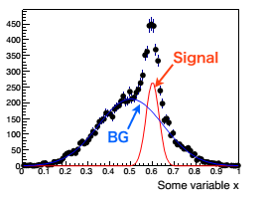
\includegraphics[width=0.6\linewidth]{./figures/likelihood_event_selection.png}
  \caption{
    In this simple cartoon model, we see a background distribution, with some
    signal of interest (the large peak). In traditional side-band analyses, cuts
    are performed around this peak to obtain a signal to background ratio.
    However, the likelihood cut method involves modeling the distribution of
    background events (blue curve) and signal events (red curve) in order to
    determine the likelihood that a given event is signal or background.
  }
  \label{fig:simple_likelihood_event_selection}
\end{figure}

\begin{figure}[ht]
  \centering
  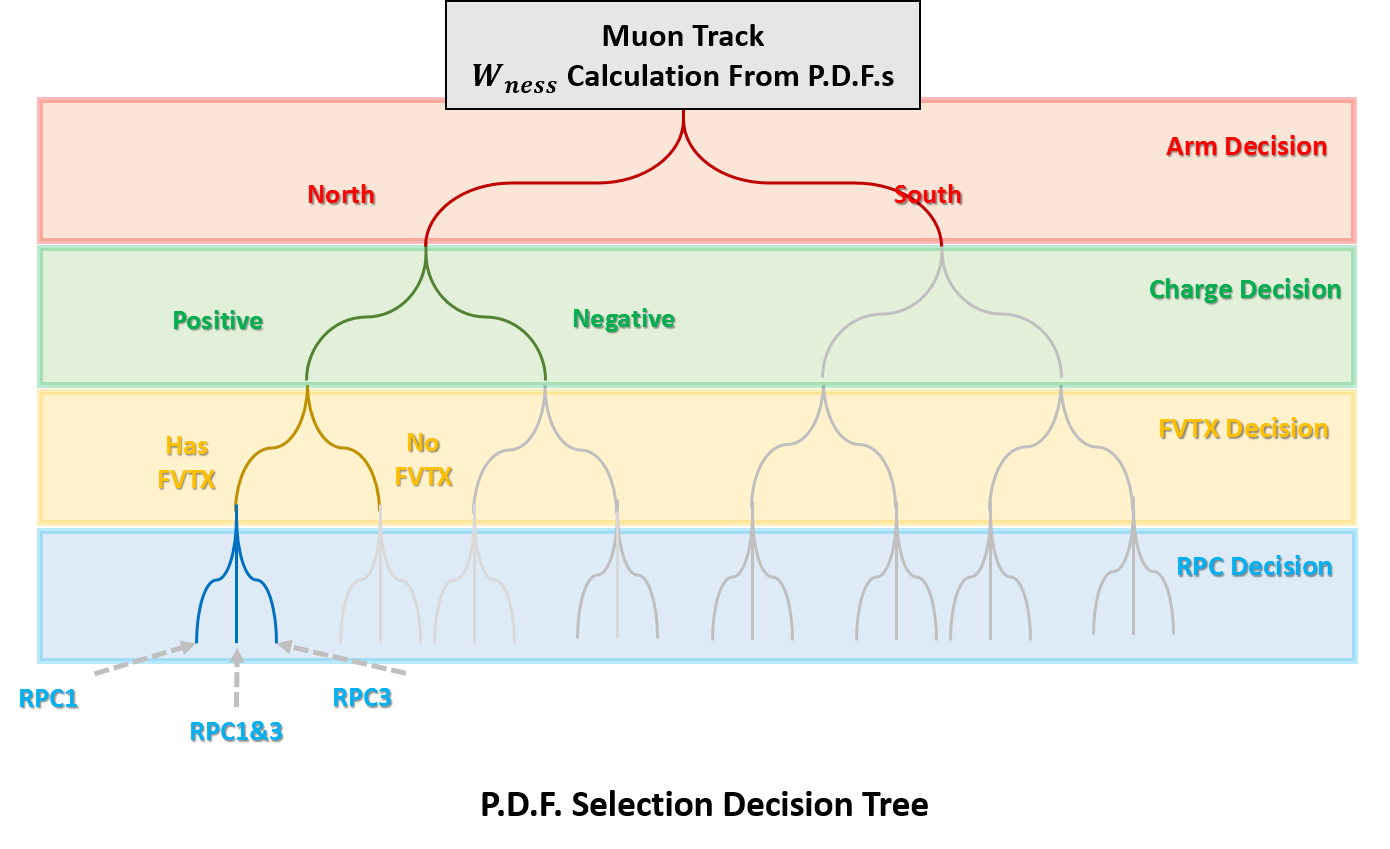
\includegraphics[width=\linewidth]{./figures/pdf_selection_tree.png}
  \caption{
    A cartoon of the decision tree to determine the PDF cocktail to use for
    quantifying the $W_{ness}$ of a given track. The track's properties are used
    to traverse the tree, and select the cocktail contents.
  }
  \label{fig:pdf_selection_tree}
\end{figure}

\clearpage
\subsection{Extended Unbinned Maximum Likelihood Selection: The Signal to
Background Ratio}
\label{sec:sbr}

\subsubsection{Extrapolation of $dw_{23}$ To Fit Region}

\begin{equation} \label{eq:dw23_wness_part}
  f(W_{ness}) = 
  P_8 + P_9 W_{ness} + 
  P_{10} {W_{ness}}^2 +
  P_{11} + {W_{ness}}^3 +
  P_{12} + {W_{ness}}^4
\end{equation}

\begin{align}\label{eq_dw23_equations}
  \sigma_1 &= P_1 + P_3 \times W_{ness} &  C_g &= P_6 + P_7 \times W_{ness} \\
  \sigma_2 &= P_4 + P_5 \times W_{ness} &  \mu &= P_0 + P_1 \times W_{ness}
\end{align}

\begin{equation}
  g(W_{ness},dw_{23}) = C_w \times 
  \left(
    \left( 
      { {1}\over{\sqrt{2\pi}\sigma_1+C_g\sqrt{2\pi}\sigma_2} }
    \right) 
    \times
    \left(
      e^{{{1}\over{2}}{\left({dw_{23-\mu}}\over{\sigma_1}\right)^2}}
        +C_ge^{{{1}\over{2}}{\left({dw_{23-\mu}}\over{\sigma_2}\right)^2}} 
    \right) 
  \right)
  \label{eq:dw23_parameterization}
\end{equation}

\begin{equation}
  F(W_{ness},dw_{23}) = f(W_{ness})\times g(W_{ness},dw_{23}) 
  \label{eq:dw23_final_parameterization}
\end{equation}

